

\StartOf{Lecture 6}

\Today{(0) Nyquist Filtering, (1) QAM, (2) PSK}

\announcements{
\begin{itemize}
  \item For today: Rice Chapter 5.2, 5.3
  \item For Mon:  Proakis \& Salehi FSK sections (From page 4 ''Frequency-Shift Keying (FSK)'' through Equation (7.5.90) on page 10 of the pdf). See Canvas.  And:  Rice 5.4. 
  \item HW 2 due tomorrow (Thu) 11:59pm. 
  \item Proj.\ 1 due Mon 11:59pm.  
  \item HW 3 posted, due Wed.\ Feb.\ 12.  
  \item Keren Li has office hours today 4-5pm in the Green Hall 2120A conference room.
\end{itemize}
}

\section{Quadrature Amplitude Modulation (QAM)}

Quadrature Amplitude Modulation (QAM) is a two-dimensional
bandpass signalling method which uses the in-phase and quadrature (cosine and sine, respectively) as the two dimensions.  Thus QAM uses two basis functions.  These are:
\begin{eqnarray} \label{E:QAM_basis}
  \phi_0(t) &=& \sqrt{2} p(t) \cos(\omega_0 t) \nnn
  \phi_1(t) &=& - \sqrt{2} p(t) \sin(\omega_0 t) 
\end{eqnarray}
where $p(t)$ is a pulse shape (like the ones we've looked at
previously) with support on $T_1 \le t \le T_2$.  That is, $p(t)$ is
only non-zero within that window.

In most flow chart-type drawings of transmitters and receivers, frequency up-conversion and down-conversion are separate from pulse shaping, which is largely true to how the device operates.  The definition of the orthonormal basis in (\ref{E:QAM_basis}) specifically considers a pulse shape at a frequency $\omega_0$.  We include it here because it is \emph{critical} to see how, with the same pulse shape $p(t)$, we can have two orthogonal basis functions.  (This is not intuitive!)

We have two restrictions on $p(t)$ that makes these two basis
functions orthonormal:
\begin{itemize}
  \item $p(t)$ is unit-energy.
  \item $p(t)$ is `low pass'; that is, it has low frequency content
  compared to $\omega_0 t$.
\end{itemize}

\subsection{Showing Orthogonality}

Let's show that the basis functions are orthogonal.  Rather than assume that the waveforms are infinite in duration, let's put finite limits $T_1$ and $T_2$ on them, and say that they are zero before $T_1$ and after $T_2$.  Starting the proof, and using $\sin (2 A) = 2 \cos A \sin A$,
\begin{eqnarray}
  \intinfty{t}{\phi_0(t)\phi_1(t)}  &=&
    - \int_{T_1}^{T_2} \sqrt{2} p(t) \cos(\omega_0 t) \sqrt{2} p(t) \sin(\omega_0
    t) dt \nnn
    &=& - 2 \int_{T_1}^{T_2} p^2(t) \cos(\omega_0 t) \sin(\omega_0 t) dt \nnn
    &=& - \int_{T_1}^{T_2} p^2(t) \sin(2 \omega_0 t) dt. \nn
\end{eqnarray}

But we don't know $p(t)$, so we can't proceed.  For a simple example, let $p(t)=c$ for a constant $c$ , for $T_1 \le t \le T_2$.  Are the two bases orthogonal?
\begin{eqnarray} \label{E:constant_pulse_mid}
  \intinfty{t}{\phi_0(t)\phi_1(t)}
    &=&  - c^2 \int_{T_1}^{T_2}  \sin(2 \omega_0 t) dt \nnn
    &=&  - c^2 \left[  - \frac{\cos(2 \omega_0 t)}{2\omega_0} \right|_{T_1}^{T_2} \nnn
    &=&  - c^2 \frac{\cos(2 \omega_0 T_2) - \cos(2 \omega_0 T_1)}{2\omega_0} 
\end{eqnarray}
Next, using the relationship,
\begin{equation}
  \cos A - \cos B = -2\sin  \frac{A + B}{2}  \sin \frac{A - B}{2}, 
\end{equation}
we can write (\ref{E:constant_pulse_mid}) as,
\begin{eqnarray}
 \intinfty{t}{\phi_0(t)\phi_1(t)} 
    &=&  c^2 \frac{\sin(\omega_0 (T_2+T_1)) \sin(\omega_0 (T_2-T_1))}{\omega_0}
    \nn
\end{eqnarray}
We only need one of the sinusoids to be zero to make the functions orthogonal.  There are two cases:
\begin{enumerate}
  \item The pulse duration $T_2-T_1$ is an integer number of
  periods.  That is, $\omega_0 (T_2-T_1) = \pi k$ for some integer
  $k$.  In this case, the right $\sin$ is zero, and so the
  correlation is exactly zero.
  \item Otherwise, the numerator bounded above and below by +1 and
  -1, because it is a sinusoid.  That is,
  \[
    -\frac{c^2}{\omega_0} \le \langle \phi_0(t), \phi_1(t) \rangle \le \frac{c^2}{\omega_0}
  \]
  Typically, $\omega_0$ is a large number.  For example, frequencies $2\pi \omega_0$ could be
  in the MHz or GHz ranges.  Certainly, when we divide by numbers on the order of $10^6$ or
  $10^9$, we're going to get a very small inner product.  For
  engineering purposes, then, $\phi_0(t)$ and $\phi_1(t)$ are orthogonal.
\end{enumerate}

Finally, we can attempt the proof for the case of arbitrary pulse
shape $p(t)$.  In this case, we use the `low-pass' assumption that
the maximum frequency content of $p(t)$ is much lower than $2\pi
\omega_0$.  This assumption allows us to assume that $p^2(t)$ is
nearly constant over the course of one cycle of the carrier
sinusoid.

This is well-illustrated in Figure 5.3.1 in the Rice book (page 240).
In this figure, we see a pulse modulated by a sine wave at frequency
$2\pi\omega_0$.  Zooming in on any few cycles, you can see that the
pulse $p^2(t)$ is largely constant across each cycle.  Thus, when we
integrate $p^2(t) \sin(2 \omega_0 t)$ across one cycle, we're going
to end up with approximately zero. 

%\Solution{How many cycles are there?  Consider the period $[T_1,T_2]$.  How many times can it be divided by $\pi /\omega_0$?  Letthe integer number be
%\[
%  L = \left\lfloor \frac{(T_2-T_1)\omega_0}{\pi } \right\rfloor.
%\]
%Then each cycle is in the period, $[ T_1 + (i-1)\pi/\omega_0 , T_1 + i\pi/\omega_0 ]$, for $i=1, \ldots, L$.  Within each of these cycles, assume $p^2(t)$ is nearly constant.  Then, in the same way that the earlier integral was zero, this part of the integral is zero here. The only remainder is the remainder (partial cycle) period, $[T_1 + L\pi/\omega_0 , T_2]$. Thus
%\begin{eqnarray}
%  \langle \phi_0(t), \phi_1(t) \rangle
%    &=& p^2(T_1+L\pi/\omega_0) \int_{T_1+L\pi/\omega_0}^{T_2} \sin(2 \omega_0 t) dt
%    \nnn
%    &=& p^2(T_1+L\pi/\omega_0)\frac{\cos(2 \omega_0 T_2) - \cos(2 \omega_0 T_1 + 2\pi L)}{2\omega_0}
%    \nnn
%    &=& p^2(T_1+L\pi/\omega_0)\frac{\sin(\omega_0 (T_2+T_1)) \sin(\omega_0 (T_2-T_1))}{\omega_0}
%    \nn
%\end{eqnarray}
 %}
%Again, the inner product is bounded on either side:
%\[
%  -\frac{p^2(T_1+L\pi/\omega_0)}{\omega_0} \le \langle \phi_0(t), \phi_1(t)
%  \rangle \frac{p^2(T_1+L\pi/\omega_0)}{\omega_0}
%\]
%which for very large $\omega_0$, is nearly zero.

\subsection{Constellation}

With these two basis functions, $M$-ary QAM is defined as an
arbitrary signal set $\mba_0, \ldots, \mba_{M-1}$, where each signal
space vector $\mba_k$ is two-dimensional:
\[
  \mba_k = [a_{k,0}, a_{k,1}]^T
\]

The signal corresponding to symbol $k$ in ($M$-ary) QAM is thus
\begin{eqnarray}
 s(t) &=& a_{k,0}  \phi_0( t) + a_{k,1} \phi_1( t) \nnn
   &=& a_{k,0}  \sqrt{2} p(t) \cos(\omega_0 t) - a_{k,1} \sqrt{2} p(t) \sin(\omega_0
 t) \nnn
   &=& \sqrt{2} p(t)  \left[ a_{k,0}  \cos(\omega_0 t) - a_{k,1} \sin(\omega_0 t) \right] \nn
\end{eqnarray} Note that we could also write the signal $s(t)$ as
\begin{eqnarray}
 s(t) &=& \sqrt{2} p(t)  \mathbb{Re} \left\{ a_{k,0} e^{j\omega_0 t} + j a_{k,1} e^{j\omega_0 t} \right\} \nnn
  &=& \sqrt{2} p(t)  \mathbb{Re} \left\{ e^{j\omega_0 t} \left( a_{k,0} + j a_{k,1}\right) \right\} \nnn
\end{eqnarray}
In many textbooks, you will see them write a QAM signal in shorthand
as
\[
 s_{CB}(t) = p(t) (a_{k,0} + j a_{k,1})
\]
This is called `Complex Baseband'.  If you do the following
operation you can recover the real signal $s(t)$ as
\[
 s(t) = \sqrt{2} \mathbb{Re} \left\{ e^{j\omega_0 t} s_{SB}(t) \right\}
\]
Many other books use complex baseband notation, so I include this because you
should be able to read other books and know what they're talking
about.

Then, we can see that the signal space representation $\mba_k$ is
given by
\[
  \mba_k = [a_{k,0}, a_{k,1}]^T
\]
for $k = 0,\ldots, M-1$

\subsection{Signal Constellations}

\begin{figure}[htbp]
  \centerline{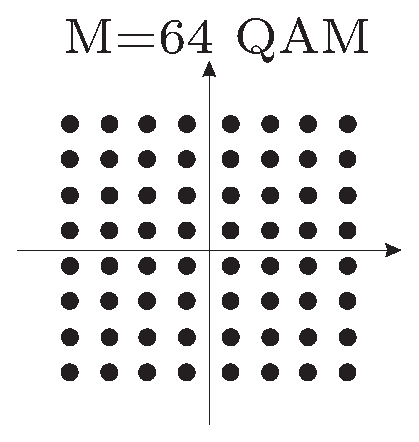
\includegraphics[width=0.3\textwidth]{../images/QAM64Eg.eps} }
  \caption{Square signal constellation for 64-QAM.}
  \label{F:QAM64Eg}
\end{figure}

\begin{itemize}
  \item See Figure 5.3.3 in the Rice book for examples of square QAM.  These
  constellations use $M = 2^{a}$ for some \textbf{even} integer $a$, and arrange
  the points in a grid.  One such diagram for $M=64$ square QAM is also given here in
  Figure \ref{F:QAM64Eg}.
  \item Figure 5.3.4 shows examples of constellations which use $M = 2^{a}$ for some \textbf{odd} integer $a$, and arrange the points in a grid.  These are either rectangular grids, or 
  squares with the corners cut out, or more hexagonal grids.
\end{itemize}

\subsection{Angle and Magnitude Representation}

You can plot $\mba_k$ in signal space and see that it has a
magnitude (distance from the origin) of $| \mba_k| = \sqrt{a_{k,0}^2
+ a_{k,1}^2}$ and angle of $\angle \mba_k =
\tan^{-1}\frac{a_{k,1}}{a_{k,0}}$.  In the continuous time signal
$s(t)$ this is
\[
s(t) = \sqrt{2} p(t) | \mba_k |  \cos(\omega_0 t + \angle \mba_k)
\]

\subsection{Average Energy in M-QAM}

The average energy is calculated as:
\begin{eqnarray}
  \En_s &=& \frac{1}{M} \sum_{i=0}^{M-1} |\mba_i|^2 \nnn
  \En_b &=& \frac{1}{M \log_2 M} \sum_{i=0}^{M-1} |\mba_i|^2 \nn
\end{eqnarray}
where $\En_s$ is the average energy per symbol and $\En_b$ is the
average energy per bit.  We'll work in class some examples of
finding $\En_b$ in different constellation diagrams.



\subsection{Phase-Shift Keying}

Some implementations of QAM limit the constellation to include only
signal space vectors with equal magnitude, \ie,
\[
  |\mba_0| = |\mba_1| = \cdots = |\mba_{M-1}|
\]
The points $\mba_i$ for $i=0, \ldots, M-1$ are uniformly spaced on
the unit circle.  Some examples are shown in Figure \ref{F:MPSKEg}.

\FigureFromAnotherLecture{
  \begin{figure}[htbp]
    \centerline{(a)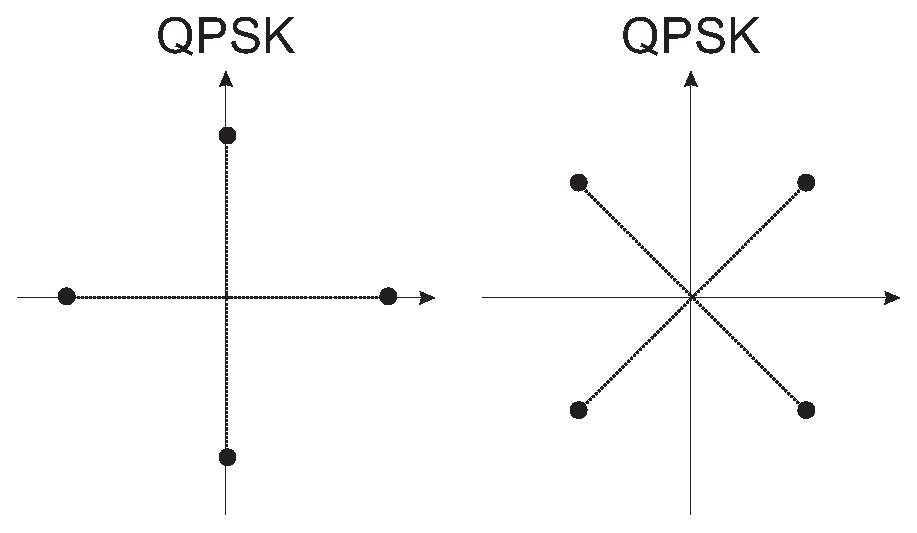
\includegraphics[width=0.6\textwidth]{../images/QPSK-signalSpaceDiagram.eps}
    }
    \centerline{(b)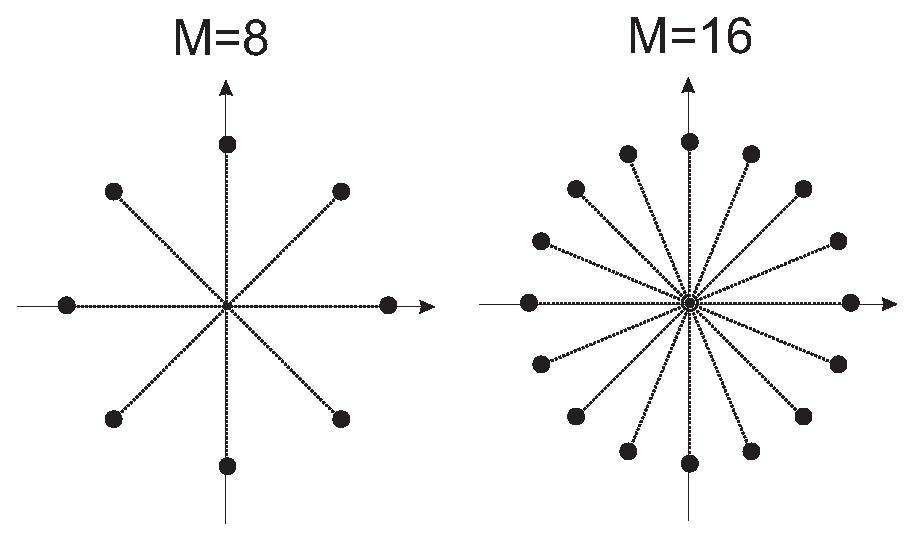
\includegraphics[width=0.6\textwidth]{../images/MPSK-signalSpaceDiagram.eps} }
    \caption{Signal constellations for (a) $M=4$ PSK and (b) $M=8$ and $M=16$ PSK.}
    \label{F:MPSKEg}
  \end{figure}
}

\paragraph{BPSK}

For example, binary phase-shift keying (BPSK) is the case of $M=2$.
Thus BPSK is the same as bipolar (2-ary) PAM.   What is the
probability of error in BPSK?  The same as in bipolar PAM, \ie, for
equally probable symbols,
\[
    \PR{\mbox{error}} = \Q{ \sqrt{\frac{2\En_b }{N_0}}}.
\]

\paragraph{QPSK}

$M=4$ PSK is also called quadrature phase shift keying (QPSK), and
is shown in Figure \ref{F:MPSKEg}(a).  Note that the rotation of the
signal space diagram doesn't matter, so both `versions' are
identical in concept (although would be a slightly different
implementation).  Note how QPSK is the same as $M=4$ square QAM.

\subsection{Systems which use QAM}

See L.W.~Couch, \emph{Digital and Analog Communication Systems}, 7th ed., 2007. Also: Wikipedia, and the Rice book:
\begin{itemize}
  \item Digital Microwave Relay, various manufacturer-specific
    protocols.  6 GHz, and 11 GHz.
  \item Dial-up modems: use a $M=16$ or $M=8$ QAM constellation.
  \item DSL.  G.DMT uses multicarrier (up to 256 carriers) methods (OFDM), and on each narrowband
    (4.3kHz) carrier, it can send up to $2^{15}$ QAM (32,768 QAM).
    G.Lite uses up to 128 carriers, each with up to $2^8=256$ QAM.
  \item Cable modems.  Upstream:  6 MHz bandwidth channel, with 64
    QAM or 256 QAM.  Downstream:  QPSK or 16 QAM.
  \item 802.11a, 802.11g:  Adaptive modulation methods, use up to 64 QAM.
  \item 802.11ac, 11ax: uses up to 1024 QAM.
  \item Digital Video Broadcast (DVB): APSK used in ETSI standard.
\end{itemize}


\subsection{Bandwidth of QAM, PAM, PSK}

The bandwidth of QAM, PAM, and PSK are all determined by the bandwidth of the pulse used.  For square root-raised cosine (SRRC) pulses, the null to null bandwidth is 
\[
 B_T = \frac{1+\alpha}{T_s}
\]
where $\alpha$ is the ``rolloff'' factor or ``excess bandwidth'' parameter of the SRRC pulse.  Recall if $\alpha=0$ then the pulse shape is a rect in the frequency domain and a sinc in the time domain, and has the smallest bandwidth.  


